\documentclass[a4paper, 12pt, final, garamond]{book}
\usepackage{cours-preambule}

\raggedbottom

\makeatletter
\renewcommand{\@chapapp}{\'Electrocin\'etique -- chapitre}
\makeatother

\begin{document}
\setcounter{chapter}{5}

\chapter{Correction du TD}

\section{Notation complexe}

\begin{enumerate}
    \item Pour passer aux formes complexes, il faut s'assurer que \textbf{les
        grandeurs soient toutes exprimées en cosinus}, puisque c'est bien le
        cosinus la partie réelle d'une exponentielle complexe. Or, $\sin\theta =
        \cos(\pi/2-\theta) = \cos(\theta-\pi/2)$, donc on a~:
        \begin{align*}
            \tau \dv{u}{t} + u(t) &= E_0\cos(\wt - \pi/2)\\
            \Leftrightarrow
            \tau \dv{\uu}{t} + \uu(t) &= E_0\exr^{-\jj\pi/2}\exr^{\jwt}\\
            \Leftrightarrow
            (1+\jwt)\uu &= E_0\exr^{-\jj\pi/2}\exr^{\jwt}\\
            \Leftrightarrow
            \Aboxed{\uu &= \frac{E_0\exr^{-\jj\pi/2}\exr^{\jwt}}{1+\jwt}}
        \end{align*}
        grâce au fait qu'en complexes, dériver revient à multiplier par $\jw$.
    \item Ici, rien de particulier~: on souligne $x$ d'abord, puis on dérive en
        multipliant par $\jw$.
        \begin{align*}
            \ddot{x} +  2\lambda \dot x + \w_0^2 x(t) &= KI_m\cos\wt\\
            \Leftrightarrow
            (\jw)^2\ul{x} + 2\lambda\jw \ul{x} + \w_0{}^2 \ul{x} &=
                KI_m\exr^{\jwt}\\
            \Leftrightarrow
            \Aboxed{\ul{x} &= \frac{KI_m\exr^{\jwt}}{\w_0{}^2 - \w^2 +
                2\lambda\jw}}
        \end{align*}
\end{enumerate}

\section{Filtre de \textsc{Wien}}
\begin{enumerate}
    \item Dans la limite très hautes fréquences, les condensateurs sont
        équivalents à des fils, donc $\uu = 0$. Dans la limite très basses
        fréquences, les condensateurs sont cette fois équivalents à des
        interrupteurs ouverts. Aucun courant ne circule dans les résistances, et
        on a donc également $\uu = 0$. Selon toute vraisemblance, c'est donc
        un filtre \textbf{passe-bande}.
    \item On observe bien une résonance en tension, étant donné qu'on trouve un
        \textbf{maximum de l'amplitude pour $\w \neq 0$ et $\w \neq \infty$}.

    \item On lit \fbox{$\w_r = \SI{10}{rad.s^{-1}}$}, et on trouve les
        pulsations de coupure en traçant une droite horizontale à $H_{m,
        \max}/\sqrt{2} = \num{0.23}$ (avec $H_{m, \max} = \num{0.33}$) et en
        prenant les abscisses des intersections. On trouve alors
        \begin{gather*}
            \boxed{\w_1 = \SI{2}{rad.s^{-1}}}
            \qet
            \boxed{\w_2 = \SI{20}{rad.s^{-1}}}
            \qdonc
            \boxed{\D\w = \SI{18}{rad.s^{-1}}}
        \end{gather*}
        En effet, l'axe des abscisses est en échelle logarithmique, il faut donc
        faire attention à la lecture.
    \item Notons $\Zu_{R\parr C}$ l'impédance et $\Yu_{R\parr C}$ l'admittance
        de l'association RC parallèle. En utilisant cette impédance, on
        reconnaît un pont diviseur de tension~:
        \begin{gather*}
            \Hu
                = \frac{\uu}{\ul{e}}
                = \frac{\Zu_{R\parr C}}{\Zu_{R\parr C} + \Zu_R + \Zu_C}
            \Leftrightarrow
            \Hu = \frac{1}{1 + \left(\Zu_R + \Zu_C\right)\Yu_{R\parr C}}\\
            \Leftrightarrow
            \ul{H}
                = \frac{1}{1 + \left(R + \dfrac{1}{\jcw}\right)\Yu_{R\parr C}}
                = \frac{1}{1 + \left(R + \dfrac{1}{\jcw}\right)\left(
                    \dfrac{1}{R} + \jcw\right)}\\
            \Leftrightarrow
            \boxed{\ul{H} = \frac{1}{3+\jj\left(RC\w - \dfrac{1}{RC\w}\right)}}
        \end{gather*}
        En factorisant par 3 et en utilisant les notations introduites dans
        l'énoncé, on trouve
        \begin{gather*}
            \ul{H}
                = \frac{1/3}{1 + \dfrac{\jj}{3} \left( x - \dfrac{1}{x} \right)}
            \Leftrightarrow
            \boxed{
            \ul{H} = \frac{H_0}{1 + \jj Q \left( x - \dfrac{1}{x} \right)}}
            \qavec
            \boxed{
            \left\{
                \begin{array}{rcl}
                    H_0  & = & 1/3\\
                    \w_0 & = & \dfrac{1}{RC}\\
                    Q    & = & 1/3
                \end{array}
            \right.
            }
        \end{gather*}
        Ce qui est remarquable avec ce montage, c'est que \textbf{le facteur de
        qualité est de 1/3 peu importe les valeurs de $R$ et $C$}, tant que ce
        sont les mêmes $R$ et $C$ en série et en dérivation.
    \item Par cette étude, on trouve que $\w_r = \w_0 = \frac{1}{RC}$~; ainsi,
        on a simplement \[\boxed{RC = \SI{0.10}{Hz}}\]
\end{enumerate}

\section{Modélisation d'un haut-parleur}
\begin{enumerate}
    \item ~

        \vspace{-18pt}
        \begin{minipage}{0.43\linewidth}
            \begin{description}
                \item[Système] : masse~;
                \item[Référentiel] : $\Rc_{\rm sol} (O,x,y,t)$~;
                \item[Position de la masse] : $\OM = x\ux$~;
                \item[Longueur ressort] : $\vv{MA} = \ell\ux$~;
                \item[Longueur à vide] : $\vv{OA} = \ell_0\ux$~;
                \item[Longueur relative] :\\
                    $(\ell - \ell_0)\ux = \vv{MO} = -x\ux$.
            \end{description}
        \end{minipage}
        \hfill
        \begin{minipage}{0.57\linewidth}
            \textbf{Bilan des forces}~:
            \begin{enumerate}
                \item Poids $\Pf = -mg\uy$~;
                \item Réaction du support $\vv{R} = R\uy$~;
                \item Force de rappel du ressort\\
                    $\vv*{F}{\rm ressort} = k(\ell - \ell_0)\ux =
                    k\vv{MO} = -kx\ux$~;
                \item Force de frottement fluide $\vv{f} = -\alpha\vf =
                    -\alpha\dot{x}\ux$~;
                \item \textbf{Force excitatrice} $\Ff = KI_m\cos(\wt)\ux$.
            \end{enumerate}
        \end{minipage}

        Avec le PFD~:
        \begin{gather*}
            m\af = \Pf + \vv{R} + \Ff_{\rm ressort} + \vv{f} +\Ff\\
            \Leftrightarrow m\left(
                \begin{array}{c}
                    \DS\dv[2]{x}{t}\\
                    0
                \end{array}
            \right)
            =
            \left(
                \begin{array}{c}
                    -kx -\alpha v + KI_m\cos(\wt)\\
                    -mg + R
                \end{array}
            \right)
        \end{gather*}
        La projection sur $\uy$ montre que la réaction du support compense le poids.
        Sur l'axe $\ux$ on trouve
        \begin{gather*}
            \boxed{m \dv[2]{x}{t} + \alpha \dv{x}{t} + kx = KI_m\cos(\wt)}
        \end{gather*}
    \item Sous forme canonique, cela devient
        \begin{gather*}
            \Leftrightarrow
            \boxed{\ddot{x} + \frac{\w_0}{Q}\dot{x} + \w_0{}^2x =
                \frac{KI_m}{m}\cos(\wt)}\\
            \qavec
            \boxed{\w_0 = \sqrt{\frac{k}{m}}}
            \qet
            \boxed{Q = \frac{\sqrt{km}}{\alpha}}
        \end{gather*}
    \item On sait que pour une entrée sinusoïdale, un système aura une solution
        homogène donnant un régime transitoire et une solution particulière de
        la forme de l'entrée~: en RSF, on étudie le régime permanent où seule la
        solution particulière est conservée, et on pourra donc écrire $x(t) =
        X_m\cos(\wt+\F)$.
    \item 
        En passant en complexes,
        \begin{gather*}
            (\jw)^2\Xu + \jw\frac{\w_0}{Q}\Xu + \w_0{}^2\Xu = \frac{KI_m}{m}\\
            \Leftrightarrow
            \ul{X} =
                \frac{KI_m}{m}\times
                \frac{1}{\w_0{}^2 - \w^2 + \dfrac{\jj}{Q}\w\w_0}
            \Leftrightarrow
            \boxed{
            \ul{X} = \frac{KI_m}{m\w_0{}^2}\frac{1}{1 -
                                        \left( \dfrac{\w}{\w_0} \right)^2 +
                                        \jj\dfrac{\w}{Q\w_0}}
                    }
        \end{gather*}

    \item En réels, on trouve
        \begin{gather*}
            \boxed{
            X(\w)
                = \left| \ul{X} \right|
                = \frac{KI_m}{m\w_0{}^2}\frac{1}{
                        \sqrt{\left( 1 - \left(\dfrac{\w}{\w_0}\right)^2 \right)^2
                        + \left(\dfrac{\w}{Q\w_0}\right)^2}}
            }
        \end{gather*}
        Elle est maximale quand le dénominateur est minimal. Après calcul,
        on trouve
        \begin{itemize}[leftmargin=60pt]
            \item[$\mathbf{Q \leq 1/\sqrt{2}}$] : l'amplitude est maximale pour
                \[\boxed{\w = 0 \qet X(0) = \frac{KI_m}{m\w_0{}^2}}\]
            \item[$\mathbf{Q > 1/\sqrt{2}}$] : l'amplitude est maximale pour
                \[\boxed{\w_r = \w_0 \sqrt{1 - \frac{1}{2Q^2}} < \w_0}
                    \qet
                    \boxed{X(\w_r) = \frac{KI_m}{m\w_0{}^2}
                        \frac{Q}{\sqrt{1 - \frac{1}{4Q^2}}}}
                \]
        \end{itemize}
        De ce résultat, nous observons qu'il \textbf{n'y a pas toujours
        résonance en élongation}, et que \textbf{la résonance est d'autant
        aiguë que $\mathbf{Q}$ est élevé}.
    \item Le déplacement est en quadrature de phase si la différence de phase
        est de $\pm\pi/2$. Sur le graphique de droite, on le trouve à $\w =
        \SI{1100}{rad.s^{-1}}$. Or, c'est à $\w = \w_0$ qu'on trouve une
        quadrature de phase, puisqu'alors $\Xu$ est un imaginaire pur. Ainsi,
        \[\w_0 = \SI{1100}{rad.s^{-1}}\]
        On pourrait déterminer le facteur de qualité en trouvant que le maximum
        d'amplitude se trouve à $\w_r = \SI{900}{rad.s^{-1}}$.
\end{enumerate}

\section{Résonance d'un circuit bouchon}
\begin{enumerate}
    \item On effectue un pont diviseur de tension aux bornes de l'impédance
        équivalente de $L$ et $C$, avec $\Yu_{\eq} = \jcw + 1/\jlw$~:
        \begin{gather*}
            \Uu
                = \frac{\Zu_{\eq}}{\Zu_{\eq} + R}E_0
                = \frac{1}{1+R\Yu_{\eq}}E_0
                = \frac{E_0}{1+\jj \left( RC\w - \dfrac{R}{L\w} \right)}
        \end{gather*}
        en utilisant que $1/\jj = -\jj$.
    \item L'amplitude réelle est
        \begin{gather*}
            U = \abs{\Uu} = \frac{E_0}{\sqrt{1 + \left( RC\w - \dfrac{R}{L\w}
            \right)^2}}
        \end{gather*}
        Cette tension réelle est maximale si le dénominateur est minimal, donc
        si $\DS \left( RC\w - \frac{R}{L\w} \right) = 0$~: cela implique qu'il y
        a résonance si $\boxed{\w = \w_0 = 1/\sqrt{LC}}$. On trouve alors
        \begin{gather*}
            \boxed{U(\w_0) = U_{\max} = E_0}
        \end{gather*}
    \item On cherche $Q\w_0 = \frac{R}{L}$ et $\DS\frac{Q}{\w_0} = RC$~; on
        trouve donc
        \[\boxed{Q = R \sqrt{\frac{C}{L}}}\]
    \item On cherche donc les pulsations de coupure telles que $U(\w) =
        \frac{U_{\max}}{\sqrt{2}}$, soit
        \begin{gather*}
            U(\w) = \frac{U_{\max}}{\sqrt{2}}
            \Leftrightarrow
            \frac{E_0}{\sqrt{1 + Q^2\left( \frac{\w}{\w_0} - \frac{\w_0}{\w}
                    \right)^2}}
                =
                \frac{E_0}{\sqrt{2}}
                \Leftrightarrow
                \boxed{Q^2\left( \frac{\w}{\w_0} - \frac{\w_0}{\w} \right)^2 = 1}
        \end{gather*}
        On prend la racine carrée de cette équation, \textbf{en prenant les deux
        solutions possibles}~:
        \begin{align*}
            Q\left( \frac{\w}{\w_0} - \frac{\w_0}{\w} \right) = -1
            &\qet
            Q\left( \frac{\w}{\w_0} - \frac{\w_0}{\w} \right) = 1\\
            \Leftrightarrow
            \left( \frac{\w}{\w_0} - \frac{\w_0}{\w} \right)\times \w\w_0 =
                - \frac{\w\w_0}{Q}
            &\qet
            \left( \frac{\w}{\w_0} - \frac{\w_0}{\w} \right)\times \w\w_0 =
                \frac{\w\w_0}{Q}\\
            \Leftrightarrow
            \w^2 - \w_0{}^2 = -\frac{\w\w_0}{Q}
            &\qet
            \w^2 - \w_0{}^2 = \frac{\w\w_0}{Q}\\
            \Leftrightarrow
            \boxed{
            \w^2 + \frac{\w_0}{Q}\w - \w_0{}^2 = 0}
            &\qet
            \boxed{
            \w^2 - \frac{\w_0}{Q}\w - \w_0{}^2 = 0}\\
            \Rightarrow
            \Delta = &\frac{\w_0{}^2}{Q} + 4\w_0{}^2\\
            \Leftrightarrow
            \Delta = &\frac{\w_0{}^2}{Q^2} \left( 1 + 4Q^2 \right)\\
            \Rightarrow
            \w_{1,\pm} = -\frac{\w_0}{2Q} \pm \frac{\w_0}{2Q} \sqrt{1+4Q^2}
            &\qet
            \w_{2,\pm} = \frac{\w_0}{2Q} \pm \frac{\w_0}{2Q} \sqrt{1+4Q^2}\\
            \Leftrightarrow
            \w_{1,\pm} = \frac{\w_0}{2Q} \left(-1 \pm \sqrt{1+4Q^2}\right)
            &\qet
            \w_{2,\pm} = \frac{\w_0}{2Q} \left(1 \pm \sqrt{1+4Q^2}\right)
        \end{align*}
        De ces quatre racines, seules deux sont positives~: la solution avec $-1 -
        \sqrt{1+4Q^2}$ est évidemment négative, et celle avec $1 - \sqrt{1+4Q^2}$
        également. Ainsi, il ne nous reste que
        \begin{gather*}
            \w_1 = \frac{\w_0}{2Q} \left( \sqrt{1+4Q^2}-1 \right)
            \qet
            \w_1 = \frac{\w_0}{2Q} \left( \sqrt{1+4Q^2}+1 \right)
        \end{gather*}
        Il ne reste qu'à calculer la différence pour avoir la bande passante~:
        \begin{gather*}
            \boxed{\D\w = \w_2 - \w_1 = \frac{\w_0}{Q}}
        \end{gather*}
    \item Sur le graphique, on trouve $U_{\max} = \SI{5}{V} = E_0$. On a de plus
        $f_0 = \SI{22.5}{kHz}$ et $\D f \approx \SI{3}{kHz}$, d'où $\boxed{Q =
        \frac{f_0}{\D f} \approx \num{7.5}}$. Avec l'expression de $Q$, on isole
        $C$~:
        \begin{gather*}
            Q = R \sqrt{\frac{C}{L}}
            \Leftrightarrow
            \boxed{C = \frac{Q^2L}{R}}
            \qavec
            \left\{
                \begin{array}{rcl}
                    Q & = & \num{7.5}\\
                    L & = & \SI{1}{mH}\\
                    R & = & \SI{1}{k\Omega}
                \end{array}
            \right.\\
            \mathrm{A.N.~:}\quad
            \boxed{C = \SI{5.6e-8}{F}}
        \end{gather*}
\end{enumerate}

\section{Système à deux ressorts}
\begin{enumerate}
    \item ~

        \vspace{-18pt}
        \begin{minipage}{0.43\linewidth}
            \begin{description}
                \item[Système] : masse~;
                \item[Référentiel] : $\Rc_{\rm sol} (O,x,y,t)$~;
                \item[Position de la masse] : $\OM = x\ux$~;
                \item[Longueur ressort 1] : $x(t) - x_0(t)$~;
                \item[Longueur ressort 2] : $L-x(t)$.
            \end{description}
        \end{minipage}
        \hfill
        \begin{minipage}{0.57\linewidth}
            \textbf{Bilan des forces}~:
            \begin{enumerate}
                \item Poids $\Pf = -mg\uy$~;
                \item Réaction du support $\vv{R} = R\uy$~;
                \item Rappel du ressort 1
                    $\vv*{F}{1} = -k_1(\ell_1 - \ell_{10})\ux$~;
                \item Rappel du ressort 2
                    $\vv*{F}{2} = k_2(\ell_2 - \ell_{20})\ux$~;
                \item Force de frottement fluide $\vv{f} = -h\vf =
                    -h\dot{x}\ux$.
            \end{enumerate}
        \end{minipage}
    \item Avec le PFD, on trouve
        \begin{gather*}
            m\af = \Pf + \vv{R} + \Ff_{1} + \Ff_{2} + \vv{f}\\
            \Leftrightarrow m\left(
                \begin{array}{c}
                    \DS\dv[2]{x}{t}\\
                    0
                \end{array}
            \right)
            =
            \left(
                \begin{array}{c}
                    -k_1(\ell_1 - \ell_{10}) +k_2(\ell_2 - \ell_{20}) -h v\\
                    -mg + R
                \end{array}
            \right)
        \end{gather*}
        La projection sur $\uy$ montre que la réaction du support compense le poids.
        Sur l'axe $\ux$ on trouve
        \begin{gather*}
            \boxed{m \dv[2]{x}{t} + h \dv{x}{t}
                = -k_1(\ell_1 - \ell_{10}) +k_2(\ell_2 - \ell_{20})}
        \end{gather*}
        En développant les longueurs comme indiqué question 1, on a
        \begin{gather*}
            \boxed{m \dv[2]{x}{t} + h \dv{x}{t} =
            -k_1(x(t) -x_0(t) -\ell_{10}) + k_2(L - x(t) - \ell_{20})}
        \end{gather*}
        À l'équilibre les dérivées de $x$ sont nulles, d'où
        \begin{gather*}
            0 = -k_1(x(t) - x_0(t) - \ell_{10}) + k_2(L-x(t) -\ell_{20})
        \end{gather*}
        Ainsi, avec $x_{0, \eq}(t) = 0$ et $L = \ell_{10}+\ell_{20}$ (d'après
        l'énoncé) puis $x(t) = x_{\eq}$ (par définition), on a 
        \begin{gather*}
            0 = -k_1(x_{\eq} -0 - \ell_{10}) + k_2(\ell_{10} +
            \cancel{\ell_{20}} -x_{\eq} -\cancel{\ell_{20}})\\
            \Leftrightarrow
            (k_1+k_2)(\ell_{10} - x_{\eq}) = 0
        \end{gather*}
        Comme $k_1+k_2 > 0$, on trouve
        \[\boxed{x_{\eq} = \ell_{10}}\]
    \item Cette fois-ci, on garde $x_0(t)$ dans l'équation. Il vient alors
        \begin{gather*}
            m\ddot{x} + h\dot{x} + (k_1+k_2)(x-x_{\eq})  = k_1x_0(t)
        \end{gather*}
        et en effectuant le changement de variable $X = x-x_{\eq}$, on trouve
        l'équation habituelle
        \begin{gather*}
            \boxed{m \ddot{X} + h \dot{X} + kX = KX_{0m}\cos(\wt)}
        \end{gather*}
        avec $k = k_1+k_2$.
    \item On a simplement $\Xu_0 = X_{0m}$, $\Xu = X_m\exr^{\jj\F}$ et $\Vu =
        V_m\exr^{\jj\F}$.
    \item En utilisant l'équation différentielle mais en complexes et sous forme
        canonique, on trouve
        \begin{gather*}
            (\jw)^2\Xu + \jw \frac{h}{m}\Xu + \frac{k}{m}\Xu = \frac{k_1}{m}X_{0m}
            \Leftrightarrow
            \Xu =
                \frac{k_1X_{0m}}{m}\times
                \frac{1}{\dfrac{k}{m} - \w^2 + \jw \dfrac{h}{m}}
        \end{gather*}
        Étant donné que $V = \dv{X}{t}$, $\Vu = \jw\Xu$, soit
        \begin{align*}
            \Vu &= 
                \frac{k_1X_{0m}}{m}\times
                \frac{\jw}{\dfrac{k}{m} - \w^2+\jw\dfrac{h}{m}}
            \\
            \Leftrightarrow
            \Vu &= 
                \frac{k_1X_{0m}}{m}\times
                \frac{1}{\dfrac{h}{m} -\jj \dfrac{k}{m\w} + \jw}
            \\
            \Leftrightarrow
            \Vu &=
            \frac{k_1}{h - \jj \dfrac{k}{\w} + \jj m\w}X_{0m}
            \\
            \Leftrightarrow
            \Vu &=
                \frac{k_1/h}{1 + \jj \left( \dfrac{m\w}{h} - \dfrac{k}{h\w}
                \right)}\Xu_0
        \end{align*}
        Avec $Q\w_0 = \frac{k}{h}$ et $\frac{Q}{\w_0} = \frac{m}{h}$, on trouve
        bien
        \begin{gather*}
            \boxed{
                \Vu = \frac{\alpha}{1+\jj Q \left( \dfrac{\w}{\w_0} -
                \dfrac{\w_0}{\w} \right)}\Xu_0
            }
            \qavec
            \boxed{
            \left\{
                \begin{array}{rcl}
                    \alpha & = & \dfrac{k_1}{h}\\
                    \w_0   & = & \sqrt{\dfrac{k}{m}}\\
                    Q      & = & \dfrac{\sqrt{km}}{h}
                \end{array}
            \right.
            }
        \end{gather*}
    \item L'amplitude réelle de la vitesse donne
        \begin{gather*}
            V_m(\w) = \frac{\alpha}{\sqrt{1 + Q^2 \left( \dfrac{\w}{\w_0} -
            \dfrac{\w_0}{\w} \right)^2}}X_{0m}
        \end{gather*}
        qui est maximale pour $\w = \w_0$. On observe donc bien une résonance en
        vitesse pour cette pulsation, avec $V_{\max} = \alpha X_{0m}$.
\end{enumerate}

\section{Résonance d'intensité dans un circuit RLC parallèle}
\begin{enumerate}
    \item Soit $\Zu$ l'impédance équivalente à cette association, et $\Yu$ son
        admittance. On a
        \begin{gather*}
            \Yu = \frac{1}{R} + \frac{1}{\jlw} + \jcw
                = \frac{\jlw + R + (\jcw)R(\jlw)}{\jj RL\w}\\
            \Leftrightarrow
            \boxed{\Zu = \frac{\jj RL\w}{\jlw + R - RLC\w^2}}
        \end{gather*}
    \item On a $\DS \frac{\Uu_0}{\Iu_0} = \Zu$ par définition de l'impédance,
        soit $\Uu_0 = \Zu\Iu_0 = \Zu I_0$ (étant donné que l'intensité n'a pas
        de phase à l'origine). Ainsi
        \begin{gather*}
            \Uu_0 = \frac{I_0\jj RL\w}{\jlw + R - RLC\w^2}
        \end{gather*}
        On rend cette équation plus lisible en mettant le dénominateur sous une
        forme adimensionnée en divisant par $\jlw$, ce qui donne
        \begin{gather*}
            \Uu_0 = \frac{RI_0}{1 + \dfrac{R}{\jlw} + \jj RC\w}
            \Leftrightarrow
            \boxed{\Uu_0 = \frac{RI_0}{1 + \jj \left( RC\w - \frac{R}{L\w} \right)}}
        \end{gather*}
    \item L'amplitude réelle est
        \begin{gather*}
            U = \abs{\Uu_0} = \frac{RI_0}{\sqrt{1 + \left( RC\w - \dfrac{R}{L\w}
            \right)^2}}
        \end{gather*}
        Cette tension réelle est maximale si le dénominateur est minimal, donc
        si $\DS \left( RC\w - \frac{R}{L\w} \right) = 0$~: cela implique qu'il y
        a résonance si $\boxed{\w = \w_0 = 1/\sqrt{LC}}$. On trouve alors
        \begin{gather*}
            \boxed{U(\w_0) = U_{\max} = E_0}
        \end{gather*}
    \item On cherche à faire apparaître $\w_0$ dans l'écriture de $U$~:
        \begin{align*}
            RC\w - \frac{R}{L\w}
                & = R\w \frac{C\sqrt{L}}{\sqrt{L}} -
                    \frac{R}{\w}\frac{\sqrt{C}}{\sqrt{C}L}
                & = R\w \sqrt{\frac{C}{L}} \frac{1}{\w_0} -
                    \frac{R}{\w} \sqrt{\frac{C}{L}} \w_0
                & = R \sqrt{\frac{C}{L}} \left( x - \frac{1}{x} \right)
        \end{align*}
        En nommant $Q = \DS R \sqrt{\frac{C}{L}}$, on obtient finalement
        \begin{gather*}
            \boxed{\Uu_0 = \frac{RI_0}{1+\jj Q \left( x - \dfrac{1}{x} \right)}}
            \qsoit
            \boxed{U = \frac{RI_0}{\sqrt{1 + Q^2\left( x - \dfrac{1}{x}
            \right)^2}}}
        \end{gather*}
        On trace pour différentes valeurs de $Q$, et on obtient~:
        \begin{center}
            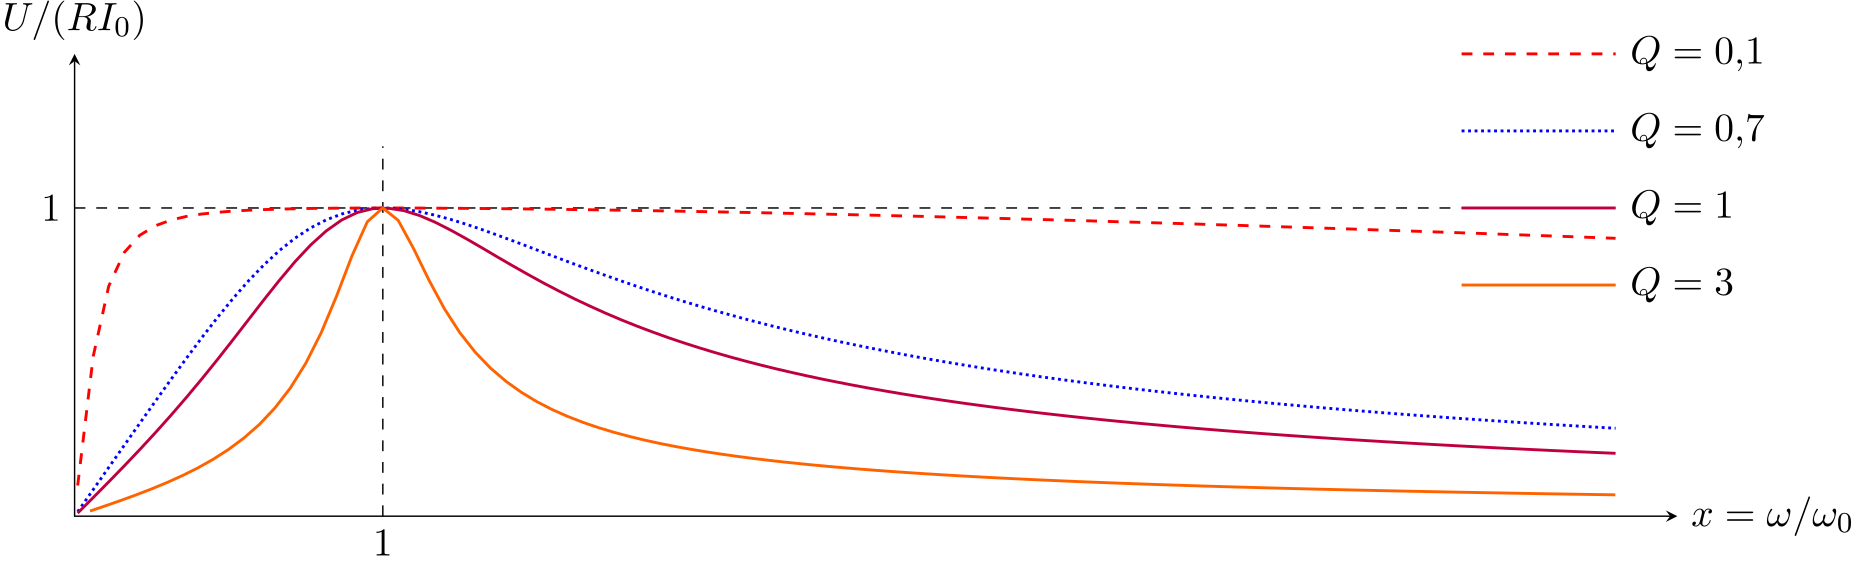
\includegraphics[width=.8\linewidth]{rlc_parr-gain}
        \end{center}
    \item On cherche donc les pulsations de coupure telles que $U(\w) =
        \frac{U_{\max}}{\sqrt{2}}$, soit
        \begin{gather*}
            U(\w) = \frac{U_{\max}}{\sqrt{2}}
            \Leftrightarrow
            \frac{RI_0}{\sqrt{1 + Q^2\left( \dfrac{\w}{\w_0} - \dfrac{\w_0}{\w}
                    \right)^2}}
                =
                \frac{RI_0}{\sqrt{2}}
                \Leftrightarrow
                \boxed{Q^2\left( \frac{\w}{\w_0} - \frac{\w_0}{\w} \right)^2 = 1}
        \end{gather*}
        On prend la racine carrée de cette équation, \textbf{en prenant les deux
        solutions possibles}~:
        \begin{align*}
            Q\left( \frac{\w}{\w_0} - \frac{\w_0}{\w} \right) = -1
            &\qet
            Q\left( \frac{\w}{\w_0} - \frac{\w_0}{\w} \right) = 1\\
            \Leftrightarrow
            \left( \frac{\w}{\w_0} - \frac{\w_0}{\w} \right)\times \w\w_0 =
                - \frac{\w\w_0}{Q}
            &\qet
            \left( \frac{\w}{\w_0} - \frac{\w_0}{\w} \right)\times \w\w_0 =
                \frac{\w\w_0}{Q}\\
            \Leftrightarrow
            \w^2 - \w_0{}^2 = -\frac{\w\w_0}{Q}
            &\qet
            \w^2 - \w_0{}^2 = \frac{\w\w_0}{Q}\\
            \Leftrightarrow
            \boxed{
            \w^2 + \frac{\w_0}{Q}\w - \w_0{}^2 = 0}
            &\qet
            \boxed{
            \w^2 - \frac{\w_0}{Q}\w - \w_0{}^2 = 0}\\
            \Rightarrow
            \Delta = &\frac{\w_0{}^2}{Q} + 4\w_0{}^2\\
            \Leftrightarrow
            \Delta = &\frac{\w_0{}^2}{Q^2} \left( 1 + 4Q^2 \right)\\
            \Rightarrow
            \w_{1,\pm} = -\frac{\w_0}{2Q} \pm \frac{\w_0}{2Q} \sqrt{1+4Q^2}
            &\qet
            \w_{2,\pm} = \frac{\w_0}{2Q} \pm \frac{\w_0}{2Q} \sqrt{1+4Q^2}\\
            \Leftrightarrow
            \w_{1,\pm} = \frac{\w_0}{2Q} \left(-1 \pm \sqrt{1+4Q^2}\right)
            &\qet
            \w_{2,\pm} = \frac{\w_0}{2Q} \left(1 \pm \sqrt{1+4Q^2}\right)
        \end{align*}
        De ces quatre racines, seules deux sont positives~: la solution avec $-1 -
        \sqrt{1+4Q^2}$ est évidemment négative, et celle avec $1 - \sqrt{1+4Q^2}$
        également. Ainsi, il ne nous reste que
        \begin{gather*}
            \w_1 = \frac{\w_0}{2Q} \left( \sqrt{1+4Q^2}-1 \right)
            \qet
            \w_1 = \frac{\w_0}{2Q} \left( \sqrt{1+4Q^2}+1 \right)
        \end{gather*}
        Il ne reste qu'à calculer la différence pour avoir la bande passante~:
        \begin{gather*}
            \boxed{\D\w = \w_2 - \w_1 = \frac{\w_0}{Q}}
        \end{gather*}
    \item $\w_0/\D\w$ est directement $Q$, donc on a
        \begin{gather*}
            A_c = Q = R \sqrt{\frac{C}{L}}
            \qavec
            \left\{
                \begin{array}{rcl}
                    R & = & \SI{7}{\Omega}\\
                    L & = & \SI{1.2e-8}{H}\\
                    C & = & \SI{2.3e-10}{F}
                \end{array}
            \right.\\
            \mathrm{A.N.~:}\quad
            \boxed{A_c = \num{5.2}}
        \end{gather*}
        L'acuité augmente avec la résistance~: c'est normal puisque la
        résistance est en parallèle du circuit, donc une absence de résistance
        signifie ici $R$ infinie (pour qu'aucun courant ne la traverse).
\end{enumerate}

\section{Condition de résonance}
\begin{enumerate}
    \item Soit $\Zu$ l'impédance équivalent à l'association en parallèle de $R$
        et $C$. On a
        \begin{gather*}
            \Zu = \frac{R/\jcw}{R + 1/\jcw} = \frac{R}{1+\jj RC\w}
        \end{gather*}
        En utilisant un pont diviseur de tension, on trouve
        \begin{gather*}
            \uu = \frac{\Zu}{\Zu + \jlw}\eu
                = \frac{1}{1+\jlw/\Zu}\eu\\
            \Leftrightarrow
            \uu = \frac{\eu}{1+ \jj \frac{L\w}{R} - LC\w^2}
                = \frac{\eu}{1+ 2\jj\xi x - x^2}
        \end{gather*}
    \item L'amplitude réelle est
        \begin{gather*}
            U = \abs{\uu} = \frac{E_0}{\sqrt{(1-x)^2 + (2\xi x)^2}}
        \end{gather*}
    On trouve le maximum de cette amplitude quand le dénominateur est
    \textbf{non nul} et minimal, c'est-à-dire
    \begin{gather*}
        U(\w_r) = U_{\max}
        \Leftrightarrow
        \left( 1 - x^2 \right)^2 + \left(2\xi x\right)^2 \text{minimal}
    \end{gather*}
    Soit $X = x^2$, et $f(X) = \left(1 - X\right)^2 + 4\xi^2X$, la fonction que
    l'on cherche à minimiser~: on cherche donc quand est-ce que sa dérivée est
    nulle, c'est-à-dire
    \begin{gather*}
        f'(X_r) = 0
        \Leftrightarrow
        -2 \left( 1-X_r \right) + 4\xi^2 = 0
        \Leftrightarrow
        X_r-1 = - 2\xi^2
        \Leftrightarrow
        X_r = 1 - 2\xi^2\\
        \Leftrightarrow
        \boxed{
        \w_r = \w_0 \sqrt{1 - 2\xi^2}}
    \end{gather*}
    ce qui n'est défini \textbf{que si} $\xi < \frac{1}{\sqrt{2}}$. Ainsi,
    \begin{itemize}[leftmargin=60pt]
        \item[$\mathbf{\xi \geq 1/\sqrt{2}}$] : \textbf{pas de résonance},
            l'amplitude est maximale pour
            \[\boxed{\w = 0 \qet U(0) = E_0}\]
        \item[$\mathbf{\xi < 1/\sqrt{2}}$] : l'amplitude est maximale pour
            \[\boxed{\w_r = \w_0 \sqrt{1 - 2\xi^2} < \w_0}\]
    \end{itemize}
\end{enumerate}

\end{document}
